\documentclass[25pt, a1paper, portrait]{tikzposter}
\usepackage[T1]{fontenc}
\usepackage{lmodern}
\usepackage[french]{babel}
\usepackage{amsmath}
\usepackage{graphicx}
\usepackage{booktabs}

\title{{{TITLE}}}
\author{{{AUTHOR}}}
\institute{Département, Établissement}

\usetheme{Simple}
\usecolorstyle{Denmark}

\begin{document}

\maketitle

\begin{columns}
  \column{0.5}

  \block{Introduction}{
    L'affiche présente un travail en un coup d'\oe il: la question, la
    méthode, les résultats et la conclusion. Chaque encadré est une
    commande \texttt{\textbackslash block}.
  }

  \block{Objectifs}{
    \begin{enumerate}
      \item Formuler la question étudiée;
      \item Proposer une méthode pour y répondre;
      \item Mesurer la qualité des résultats.
    \end{enumerate}
  }

  \block{Méthode}{
    Le modèle étudié s'écrit
    \[
      \frac{\mathrm{d}x}{\mathrm{d}t} = -\lambda x, \qquad x(0) = x_0.
    \]
    \begin{itemize}
      \item Première étape de la méthode;
      \item Deuxième étape;
      \item Troisième étape.
    \end{itemize}
  }

  \column{0.5}

  \block{Résultats}{
    \begin{tikzfigure}[Une image du projet: remplacez-la par la vôtre.]
      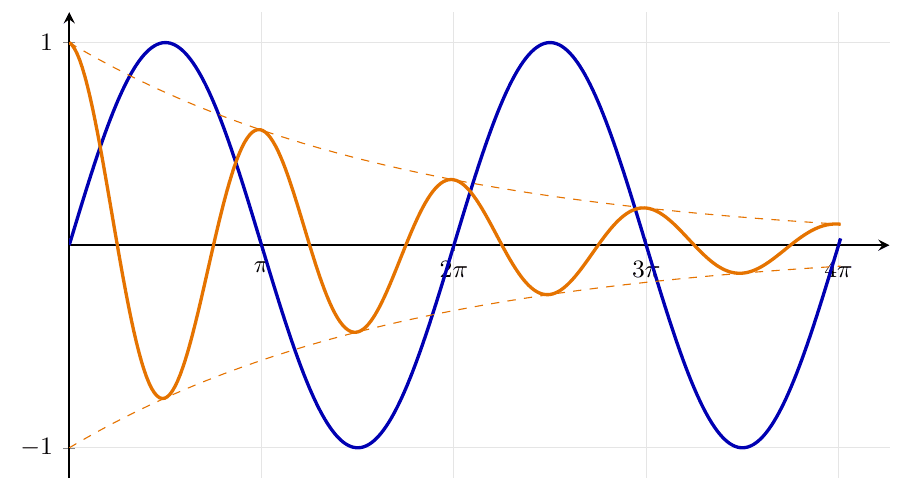
\includegraphics[width=0.9\linewidth]{images/courbes.png}
    \end{tikzfigure}
    \vspace{1em}
    \begin{center}
      \begin{tabular}{lcc}
        \toprule
        Essai & $\lambda$ & Erreur (\%) \\
        \midrule
        1 & 0,182 & 1,1 \\
        2 & 0,179 & 0,6 \\
        \bottomrule
      \end{tabular}
    \end{center}
  }

  \block{Discussion}{
    La discussion compare les résultats aux travaux antérieurs et en
    précise les limites.
  }

  \block{Conclusion}{
    La conclusion rappelle le message principal en une ou deux phrases.
  }
\end{columns}

\block{Références}{
  \small
  D.~E. Knuth, \emph{The \TeX book}, Addison-Wesley, 1984.
}

\end{document}
